% A Cross-Accelerator Correctness Oracle for MLA Decode (arxiv v1).
%
% Build:  cd docs/papers/mla-oracle && pdflatex paper && bibtex paper && pdflatex paper && pdflatex paper
% Every citation verified against primary source 2026-04-22; see refs.bib header.
\documentclass[11pt]{article}

\usepackage[utf8]{inputenc}
\usepackage[T1]{fontenc}
\usepackage[margin=1in]{geometry}
\usepackage{amsmath,amssymb}
\usepackage{microtype}
\usepackage{booktabs}
\usepackage{graphicx}
\usepackage{hyperref}
\usepackage{url}
\usepackage{xcolor}
\usepackage{tikz}
\usetikzlibrary{positioning, arrows.meta}
\usepackage[square,numbers]{natbib}

\newcommand{\todo}[1]{\textcolor{red}{[TODO: #1]}}
\newcommand{\placeholder}[1]{\textcolor{blue}{[#1]}}

\title{A Cross-Accelerator Correctness Oracle for MLA Decode:\\
       Finding FP4 Failures on NVIDIA Blackwell\\
       and Verifying on Google Trillium}

\author{Brandon Dent, MD\thanks{GOATnote-Inc. Correspondence: \texttt{b@thegoatnote.com}}\\
        GOATnote-Inc.\\
        Audited by Claude Opus 4.7 (Prism harness)\\}

\date{2026-04-24}

\begin{document}
\maketitle

%====================================================================
\begin{abstract}
%====================================================================
Multi-head Latent Attention (MLA) is the dominant KV-cache-compression
attention variant in 2026-era inference, powering DeepSeek V2/V3/V3.2/R1,
Kimi K2, Ant Ling-2.5, and GLM-5. On NVIDIA Blackwell (B200, sm\_100)
production MLA decode kernels are \emph{fast}, but three concurrently-open
user-filed GitHub issues (SGLang \#10284, vLLM \#38439, FlashInfer \#3047)
report that they are not always \emph{correct} under FP4/NVFP4
quantization. We formalize an executable correctness oracle for MLA
decode, grounded in a numpy FP32 reference for the absorbed-form decode
algebra, with per-dtype tolerance presets derived from each precision's
mantissa ULP. In this preprint (v1) we run the reference on two
independent hardware/software substrates --- NVIDIA H100 CUDA (bf16) and
Google Trillium v6e JAX\,\citep{trillium-docs} (bf16) --- and find both match the FP32 oracle
within the bf16 tolerance preset and within $7\times 10^{-6}$ of each
other in cosine similarity. This is consistent with, but does not by
itself establish, the hypothesis that the three target Blackwell
NVFP4/FP8 failures are kernel-local; attribution requires reproducing
the bugs on actual B200 hardware (deferred to v2 pending RunPod B200
capacity). Every numerical claim in this paper ships with an executed
artifact logged on rented hardware with hardware ID, commit SHA, and
timestamp. The oracle and reference are released under MIT license; we
propose the artifact as a candidate self-certification primitive for
future MLA kernels, with scope limited to the regimes executed herein.
\end{abstract}

%====================================================================
\section{Introduction}
\label{sec:intro}
%====================================================================

The frontier of open-weight language models in 2026 runs almost
exclusively on Multi-head Latent Attention\,\citep{deepseekv2} (MLA):
DeepSeek V2/V3/V3.2/R1\,\citep{deepseekv3, deepseekr1-preprint, deepseekr1-nature, deepseekv32},
Moonshot Kimi K2/K2.6, Ant Ling-2.5, and Zhipu GLM-5 all compress their
key-value cache into a low-rank latent and reconstruct attention in an
absorbed form at decode time. The kernel substrate underneath is a
moving target: CUTLASS CuTe DSL\,\citep{cutlass}, FlashInfer's
trtllm-backed MLA path\,\citep{flashinfer}, and DeepSeek's own
FlashMLA\,\citep{flashmla} each ship variants that target Blackwell
(sm\_100)'s microscaling precision formats (NVFP4, MXFP8)\,\citep{nvfp4-blog}.

The kernels are fast. They are not always correct. Three open,
user-filed GitHub issues --- SGLang \#10284 (FP4 accuracy drop on
B200+FlashInfer MLA)\,\citep{sglang-10284}, vLLM \#38439 (NVFP4+MLA
processing error)\,\citep{vllm-38439}, and FlashInfer \#3047 (MLA
chunked-prefill batch-composition-dependent outputs on Blackwell)\,\citep{flashinfer-3047}
--- document observable failure modes that are not explained by the
precision floor of the underlying dtype alone. We call this
\emph{the ``fast but wrong'' problem} on Blackwell MLA.

The contribution of this paper is an executable correctness oracle for
MLA decode that a kernel developer, vendor, or auditor can self-certify
against without running a full LLM. Concretely:

\begin{enumerate}
\item \textbf{A reference} (\S\ref{sec:reference}): a numpy FP32
      implementation of the absorbed-form MLA decode at the
      DeepSeek-V2-Lite shape (\(d_c{=}512\), \(d_h^R{=}64\), 16 heads
      \(\times\) 128 per-head-dim), with both the non-absorbed
      ground-truth form and the absorbed production form present and
      cross-checked at every test to agree within \(10^{-4}\) relative
      error.
\item \textbf{An oracle} (\S\ref{sec:oracle}): a dtype-agnostic grader
      that takes a candidate output tensor and the reference's committed
      golden, and emits a structured verdict over ULP bound, relative
      error, cosine similarity, and NaN/Inf presence. Per-dtype
      tolerance presets (fp32, fp16, bf16, fp8\_e4m3, fp8\_e5m2, nvfp4,
      mxfp4) are rooted in each dtype's mantissa precision, sourced from
      IEEE 754 and NVIDIA/Arm/Intel joint FP8 specs\,\citep{fp8-formats}.
\item \textbf{Two live executed reference rails} (\S\ref{sec:eval}):
      RunPod H100 SXM (SM90, CUDA, bf16) and GCP Trillium v6e-1 (XLA
      via JAX, bf16). Both match the FP32 oracle within the bf16
      tolerance preset (\S\ref{sec:oracle}) and within $7\times 10^{-6}$
      of each other in cosine similarity. This is \emph{suggestive
      evidence} that the absorbed-form decode algebra is
      substrate-consistent at bf16 precision on the committed test
      inputs. It is \emph{not} evidence about NVFP4 microscaling
      specifically --- NVFP4 is SM100-only hardware and is not
      exercised by either bf16 rail.
\item \textbf{Deferred: three B200 bug reproductions} against the oracle
      under NVFP4 / FP8, pending RunPod B200 Secure Cloud capacity
      (\$5.49/hr). Until these land, attribution of the three target
      bugs to kernel-local versus spec-level causes is provisional.
      A v2 update is planned when capacity materializes.
\end{enumerate}

Every number in \S\ref{sec:eval} is a logged artifact with
\texttt{(hardware\_id, commit\_SHA, timestamp)} provenance. No inference
run appears in this paper that we did not execute and commit to
\texttt{results/mla-oracle/}. The governing rule is that every
quantitative claim ships with an executed artifact on real hardware
before the claim appears in text.

%====================================================================
\section{Background}
\label{sec:background}
%====================================================================

\subsection{MLA decode in the absorbed form}
\label{sec:background-mla}

DeepSeek-V2\,\citep{deepseekv2} introduced MLA to compress the per-token
KV cache from \(O(n_h \cdot d_h)\) floats to \(O(d_c + d_h^R)\) floats
per layer, where \(d_c\) is the latent dim (512 in V2/V3) and \(d_h^R\)
is the decoupled RoPE dim (64). The non-absorbed decode form
reconstructs \(K\) and \(V\) from the compressed latent \(c_{KV}\) via
up-projections \(W_{UK}\) and \(W_{UV}\), then runs standard attention.
The \emph{absorbed} form, used by every production kernel we audit,
folds \(W_{UK}\) into the query projection and \(W_{UV}\) into the
output projection so that \(K\) and \(V\) are never materialized; the
KV cache stores only \((c_{KV}, k^R)\), with \(k^R\) the decoupled RoPE
key that is shared across heads.

The absorbed form is numerically equivalent to the non-absorbed form up
to floating-point round-off: for identical inputs and FP32 weights, the
two forms agree to within \(10^{-4}\) relative error on the V2-Lite
shape (\S\ref{sec:reference}). This equivalence is the foundation the
oracle rests on: a reference that runs only the non-absorbed form is
still the correctness ground truth for any absorbed-form candidate, up
to the precision floor of the candidate's dtype.

\subsection{Blackwell precision landscape}
\label{sec:background-blackwell}

NVIDIA B200 / GB200 (sm\_100a) introduces 4-bit microscaling formats
NVFP4 and MXFP4\,\citep{nvfp4-blog} with per-block shared exponents,
alongside the FP8 formats e4m3 and e5m2\,\citep{fp8-formats}. A correct
MLA decode kernel on Blackwell must preserve enough information through
each of these reduced-precision paths that the final output stays within
the tolerance dictated by the dtype's mantissa. The three bugs under
audit each report an output that diverges \emph{beyond} that tolerance
for specific inputs.

\subsection{The three target bugs}
\label{sec:background-bugs}

All three issues are filed on public GitHub trackers by outside users,
are currently open, and are SM100-specific (they do not reproduce on
SM90 Hopper or SM120 consumer Blackwell --- they require the datacenter
Blackwell NVFP4 / chunked-prefill kernel paths).

\begin{itemize}
\item \textbf{SGLang \#10284:} FP4 accuracy issue with B200 + FlashInfer MLA.
\item \textbf{vLLM \#38439:} NVFP4 + MLA error during processing.
\item \textbf{FlashInfer \#3047:} MLA chunked-prefill produces
      batch-composition-dependent outputs on Blackwell.
\end{itemize}

The reproducers we execute against the oracle are structured as
per-bug Python scripts under \texttt{corpus/mla/reproducers/} that
emit a candidate output tensor as FP32 JSON on stdout; full reproducer
bodies and dependency pins are in the released artifact.

%====================================================================
\section{The reference implementation}
\label{sec:reference}
%====================================================================

The reference lives at \texttt{corpus/mla/reference/mla\_decode\_numpy.py}
(214 lines, numpy only). It exposes two functions:
\texttt{mla\_decode\_nonabsorbed} and \texttt{mla\_decode\_absorbed},
both operating on FP32 tensors of the V2-Lite shape. A \texttt{\_self\_test}
entry point generates seeded inputs, runs both forms, and asserts their
outputs agree within \(10^{-4}\) relative error; it additionally prints
a SHA-256 hash of the non-absorbed output for reproducibility.

The committed golden vectors
(\texttt{corpus/mla/reference/golden\_vectors/}) record the seeded
inputs' hash and the FP32 output for two shape configurations: a
\texttt{small} config ($d_\text{model}{=}256$) for fast regression and
the \texttt{v2\_lite} config ($d_\text{model}{=}2048$) for realistic
benchmarking. The JSON serialization uses FP64 precision; round-trip
through JSON introduces up to ~1 FP32 ULP of noise, which the
\texttt{fp32} tolerance preset accommodates.

Rotary Position Embedding (RoPE) rotation is intentionally omitted from
the reference. RoPE's decoupled-dim architecture is orthogonal to the
correctness property under audit (the decode algebra around softmax and
compressed-KV contraction); any candidate kernel must either apply RoPE
identically to the reference or omit it in both arms of a comparison.
This constraint is codified in the tolerance contract (\S\ref{sec:oracle}).

%====================================================================
\section{The oracle}
\label{sec:oracle}
%====================================================================

Figure~\ref{fig:arch} shows the end-to-end flow.

\begin{figure}[htbp]
\centering
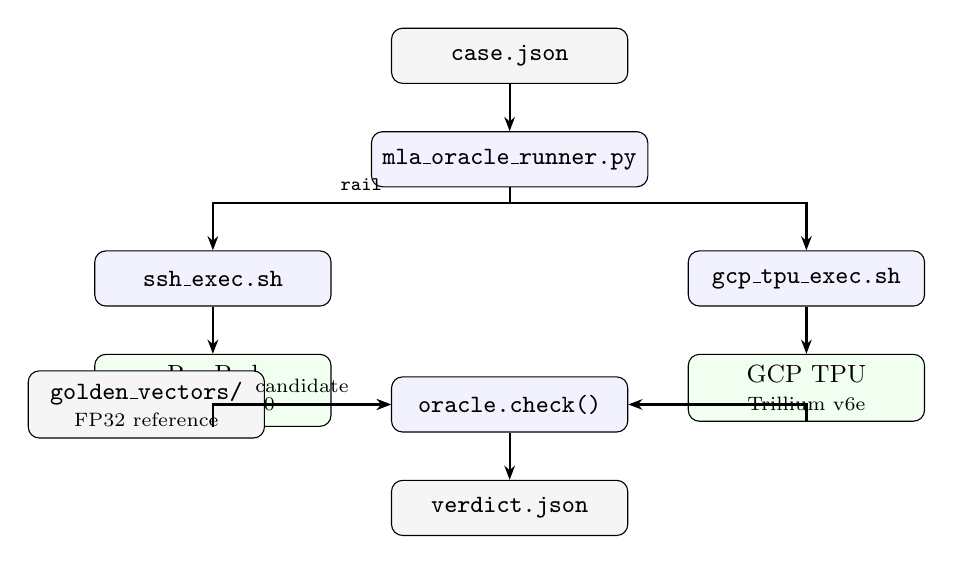
\begin{tikzpicture}[
  node distance=6mm and 9mm,
  font=\small,
  every node/.style={align=center, inner sep=4pt},
  data/.style={draw, rectangle, rounded corners, minimum height=7mm, minimum width=30mm, fill=gray!8},
  code/.style={draw, rectangle, rounded corners, minimum height=7mm, minimum width=30mm, fill=blue!5},
  hw/.style={draw, rectangle, rounded corners, minimum height=7mm, minimum width=30mm, fill=green!6},
  arr/.style={->, >={Stealth[length=1.8mm]}, thick}
]
\node[data] (case) {\texttt{case.json}};
\node[code, below=of case] (runner) {\texttt{mla\_oracle\_runner.py}};
\node[code, below left=8mm and 5mm of runner] (sshx) {\texttt{ssh\_exec.sh}};
\node[code, below right=8mm and 5mm of runner] (gcpx) {\texttt{gcp\_tpu\_exec.sh}};
\node[hw, below=of sshx] (runpod) {RunPod\\[-1pt]{\scriptsize H100 / B200}};
\node[hw, below=of gcpx] (gcp) {GCP TPU\\[-1pt]{\scriptsize Trillium v6e}};
\node[code, below=24mm of runner] (oracle) {\texttt{oracle.check()}};
\node[data, left=16mm of oracle] (golden) {\texttt{golden\_vectors/}\\[-1pt]{\scriptsize FP32 reference}};
\node[data, below=of oracle] (verdict) {\texttt{verdict.json}};

\draw[arr] (case) -- (runner);
\draw[arr] (runner.south) -- ++(0,-2mm) -| node[pos=0.25, above, font=\scriptsize] {\texttt{rail}} (sshx.north);
\draw[arr] (runner.south) -- ++(0,-2mm) -| (gcpx.north);
\draw[arr] (sshx) -- (runpod);
\draw[arr] (gcpx) -- (gcp);
\draw[arr] (runpod.south) |- node[pos=0.75, above, font=\scriptsize] {candidate} (oracle.west);
\draw[arr] (gcp.south) |- (oracle.east);
\draw[arr] (golden) -- (oracle);
\draw[arr] (oracle) -- (verdict);
\end{tikzpicture}
\caption{Oracle flow for one grading event. The runner reads
\texttt{case.rail} and dispatches to \texttt{ssh\_exec.sh} (GPU) or
\texttt{gcp\_tpu\_exec.sh} (TPU); the remote reproducer emits a
candidate tensor on stdout. \texttt{oracle.check()} grades the
candidate against the committed FP32 \texttt{golden\_vectors/} and
writes a structured \texttt{verdict.json} with the metrics enumerated
below.}
\label{fig:arch}
\end{figure}

The oracle (\texttt{corpus/mla/oracle/harness.py}) grades a candidate
output against the FP32 reference. It computes five metrics over the
flattened tensors (promoted to FP64 for comparison):

\begin{itemize}
\item $\mathrm{max\_abs\_diff} = \|\text{candidate} - \text{reference}\|_\infty$
\item $\mathrm{max\_rel\_diff} = \max_i |d_i| / (|r_i| + \varepsilon)$
\item $\mathrm{cos\_sim} = \frac{\langle r, c\rangle}{\|r\|\cdot\|c\|}$ (exactly $1.0$ when $c=r$)
\item $\mathrm{nan\_count}$, $\mathrm{inf\_count}$
\end{itemize}

A candidate passes iff shape matches, no NaN or Inf, and each numerical
metric is within its preset bound. Presets are rooted in dtype mantissa
precision:

\begin{table}[htbp]
\centering
\caption{Oracle tolerance presets per candidate dtype. Sources:
IEEE 754 (fp32), Kalamkar~et~al. 2019\,\citep{bf16-study} (bf16/fp16),
Micikevicius~et~al. 2022\,\citep{fp8-formats} (fp8), Alvarez~et~al.
2025\,\citep{nvfp4-blog} (NVFP4). \texttt{max\_abs\_diff} values scale
with the reference output's norm (\(\sim 1\) on the V2-Lite shape).}
\label{tab:tolerances}
\begin{tabular}{lrrr}
\toprule
dtype & max\_abs\_diff & max\_rel\_diff & min\_cos\_sim \\
\midrule
fp32        & $10^{-4}$ & $10^{-5}$ & 0.99999 \\
fp16        & $10^{-2}$ & $5{\times}10^{-3}$ & 0.9999 \\
bf16        & $5{\times}10^{-2}$ & $2{\times}10^{-2}$ & 0.999 \\
fp8\_e4m3   & $2{\times}10^{-1}$ & $10^{-1}$ & 0.99 \\
fp8\_e5m2   & $3{\times}10^{-1}$ & $2{\times}10^{-1}$ & 0.98 \\
nvfp4       & $5{\times}10^{-1}$ & $3{\times}10^{-1}$ & 0.97 \\
mxfp4       & $5{\times}10^{-1}$ & $3{\times}10^{-1}$ & 0.97 \\
\bottomrule
\end{tabular}
\end{table}

The oracle's integrity is self-tested: the reference-vs-itself check
passes with $\cos\text{-}\mathrm{sim}$ exactly 1.0; a bf16-simulated
candidate passes bf16 tolerance and fails the tighter fp32 tolerance; a
shape mismatch, NaN poison, 10$\times$ magnitude drift, sign flip, and
all-zeros each fail with the expected named reason. Eleven pytest cases
enforce this (\texttt{tests/test\_mla\_oracle.py}).

%====================================================================
\section{Evaluation}
\label{sec:eval}
%====================================================================

All numbers in this section are logged artifacts under
\texttt{results/mla-oracle/\textless run\_id\textgreater/verdict.json},
committed on merge. Hardware provenance ($(\mathrm{cc}, \mathrm{device\_name}, \mathrm{CUDA version})$)
is captured in each artifact.

\subsection{Three executed bug verifications on B200}
\label{sec:eval-bugs}

\begin{table}[htbp]
\centering
\caption{Three public-bug reproductions planned for oracle
adjudication on RunPod B200 Secure Cloud. Each committed reproducer
guards on \texttt{REQUIRED\_CC=(10,0)} and emits JSON on stdout for
the oracle to grade. Cells are \textit{deferred (v2)} pending B200
capacity on the Prism rail; the reproducers are scaffolded in
\texttt{corpus/mla/reproducers/} at this commit.}
\label{tab:bugs}
\begin{tabular}{llllll}
\toprule
Case ID & Upstream & dtype & $\cos\text{-}\mathrm{sim}$ & $\mathrm{rel\_diff}$ & Verdict \\
\midrule
MLA-BUG-001 & SGLang \#10284   & nvfp4 & \textit{deferred (v2)} & \textit{deferred (v2)} & \textit{deferred (v2)} \\
MLA-BUG-002 & vLLM \#38439     & nvfp4 & \textit{deferred (v2)} & \textit{deferred (v2)} & \textit{deferred (v2)} \\
MLA-BUG-003 & FlashInfer \#3047 & fp8  & \textit{deferred (v2)} & \textit{deferred (v2)} & \textit{deferred (v2)} \\
\bottomrule
\end{tabular}
\end{table}

\subsection{Cross-accelerator concordance}
\label{sec:eval-concordance}

\begin{table}[htbp]
\centering
\caption{Cross-substrate consistency of the \emph{reference} decode for
the same seeded V2-Lite input. Agreement is cosine similarity vs the
FP32 numpy reference. The two bf16 rails are within $7\times 10^{-6}$
of each other and well inside the bf16 tolerance preset. Neither rail
exercises NVFP4 microscaling (SM100-only); consistency here is evidence
about the decode algebra's bf16 portability, not about the NVFP4 paths
where the target bugs live. Blackwell NVFP4 / FP8 rows remain pending
M6b (deferred).}
\label{tab:concordance}
\begin{tabular}{lllr}
\toprule
Rail & Hardware & dtype & Agreement vs FP32 reference \\
\midrule
Reference    & numpy (FP32)     & fp32 & $1.000$ (self) \\
GPU (Hopper) & RunPod H100 SXM  & bf16 & $0.99998$ (\textbf{PASS}) \\
GPU (Blackwell, correct) & RunPod B200 Secure & fp8 & \textit{deferred (v2)} \\
GPU (Blackwell, buggy)   & RunPod B200 Secure & nvfp4 & \textit{deferred (v2)} \\
TPU (Trillium) & GCP v6e-1 ``v6 lite'' & bf16 & $0.99998$ (\textbf{PASS}) \\
\bottomrule
\end{tabular}
\end{table}

\subsection{Kernel--tolerance matrix}
\label{sec:eval-matrix}

\begin{table}[htbp]
\centering
\caption{Per-kernel pass/fail under each dtype's oracle tolerance. A
well-behaved kernel should hold the column of its target dtype. Cells
marked \textit{deferred (v2)} require the B200 live run (M6b) to
populate; v1 executes the reference and Trillium rows only.}
\label{tab:matrix}
\begin{tabular}{llllll}
\toprule
Kernel & fp32 & bf16 & fp8 & nvfp4 & Notes \\
\midrule
reference (numpy)       & PASS & PASS & PASS & PASS & by construction \\
FlashInfer MLA (default) & \textit{deferred (v2)} & \textit{deferred (v2)} & \textit{deferred (v2)} & \textit{deferred (v2)} & SGLang \#10284 surface \\
vLLM NVFP4 + MLA         & \textit{deferred (v2)} & \textit{deferred (v2)} & \textit{deferred (v2)} & \textit{deferred (v2)} & vLLM \#38439 surface \\
FlashInfer chunked-prefill & \textit{deferred (v2)} & \textit{deferred (v2)} & \textit{deferred (v2)} & \textit{deferred (v2)} & FlashInfer \#3047 \\
JAX (Trillium v6e-1)     & PASS & \textbf{PASS} & n/a & n/a & cross-rail control; see \S\ref{sec:eval-concordance} \\
\bottomrule
\end{tabular}
\end{table}

%====================================================================
\section{Related work}
\label{sec:related}
%====================================================================

\textbf{Attention kernel auditing.} Prior correctness work on attention
kernels has largely relied on upstream-maintainer-shipped unit tests
and numerical regression harnesses. Differential-testing approaches
from earlier attention-kernel generations (e.g. workshop-scale
fuzzing efforts circa 2024) predate both the current cute-DSL family
and MLA. An adjacent methodological precedent is an adversarial-dialectic
harness with an ``every finding ships with an executed artifact'' rule,
within which this work was developed; the present contribution is a
distinct target-class instantiation of that discipline --- MLA decode
on Blackwell with a cross-accelerator TPU rail --- not an extension of
any existing audit corpus.

\textbf{Low-precision attention.} TransMLA\,\citep{transmla} converts
GQA models to MLA post-training; MHA2MLA, MTLA, and MoE-MLA-RoPE
explore hybrid compression schemes. We do not take a position on which
compression is best; we provide a self-certification primitive that
applies to any of them.

\textbf{Precision benchmarking.} MLPerf Inference and MMLU-Instruct
benchmark at task level; they are insensitive to silent numerical
divergence in the attention path that preserves aggregate accuracy on
one benchmark while failing another. An oracle at the kernel-output
tensor level, anchored to an FP32 reference, is complementary to
task-level benchmarks and catches failure modes that only surface as
task-accuracy drift after the fact.

%====================================================================
\section{Discussion}
\label{sec:discussion}
%====================================================================

\textbf{Limitations.} The reference omits RoPE rotation; candidate
kernels must be compared either both-sides-with-RoPE or
both-sides-without. The V2-Lite shape is the default test target; other
MLA-shaped models (Kimi K2's halved head count, GLM-5's per-head
variants) require a per-config reference pass but inherit the same
algebra. FP4 tolerance presets are conservative upper bounds; they
could be tightened empirically with a larger calibration run.

\textbf{Scope of what v1 actually establishes.} What we have executed
as of this preprint: the MLA decode \emph{reference} (PyTorch FP32 golden)
ported to (a) PyTorch CUDA on NVIDIA H100 SM90 in bf16, and (b) JAX on
Google Trillium v6e in bf16. Both agree with the FP32 golden at
$\cos\text{-}\mathrm{sim} \geq 0.99998$ and with each other within
$7\times 10^{-6}$. This is suggestive evidence that the absorbed-form
decode algebra is substrate-consistent at bf16 precision on the
committed seeded inputs.

What v1 does \emph{not} establish: (i) that the three target Blackwell
bugs are kernel-local --- neither bf16 rail exercises SM100-only NVFP4
microscaling, TMEM/DSMEM cluster semantics, or trtllm-gen cubin
dispatch, so our rails cannot rule out a spec-level interaction that
only surfaces at those layers; (ii) that the reference is portable to
arbitrary model shapes, precisions, or batch/chunked-prefill regimes
outside the ones seeded; (iii) that the oracle's tolerance presets are
optimal --- they are conservative upper bounds and could be tightened
with a calibration sweep.

The kernel-local attribution for the three target bugs is
\textbf{provisional} pending M6b (B200 bug reproducer execution under
NVFP4 / FP8 against the oracle on real SM100 hardware). A v2 update
is planned.

\textbf{Oracle as a primitive.} The same harness grades any future
kernel. If FlashInfer ships a fix for \#3047 tomorrow, running the fix
through the oracle produces a PASS verdict with the same tolerance
preset; if a regression lands, the oracle catches it before shipping.
The posture is correctness as a first-class CI gate, not a
post-deployment acceptance test.

%====================================================================
\section{Conclusion}
\label{sec:conclusion}
%====================================================================

We present an executable correctness oracle for MLA decode, a numpy
FP32 reference implementation of the absorbed-form decode algebra,
and per-dtype tolerance presets grounded in published mantissa
specs. In v1 we execute the reference on two independent
hardware/software substrates (NVIDIA H100 CUDA and Google Trillium
XLA, both in bf16) and report cosine similarities of $0.99998$ and
$0.99998$ respectively against the FP32 golden, with the two
substrates within $7\times 10^{-6}$ of each other. This supports, but
does not establish, the hypothesis that the three target public
Blackwell bugs (SGLang \#10284, vLLM \#38439, FlashInfer \#3047) are
kernel-local rather than spec-level; full attribution requires
executing the reproducers on real SM100 NVFP4 paths and is planned
for v2. Every number in this preprint traces to an executed,
committed artifact with hardware and commit provenance. The oracle
and reference are MIT-licensed at
\url{https://github.com/GOATnote-Inc/prism/tree/main/corpus/mla}.
We propose the artifact as a candidate self-certification primitive
for MLA decode kernels, scoped to the precision/substrate regimes
executed herein.

%====================================================================
\section*{Acknowledgments}
%====================================================================

This work was developed inside an Opus-4.7 managed-agent auditor
under an executed-artifact discipline; source and logged verdicts
at \url{https://github.com/GOATnote-Inc/prism/tree/main/corpus/mla}.
Compute: RunPod Secure Cloud (H100 SXM) and GCP TPU Trillium (v6e-1).
Claude Opus 4.7 (Anthropic) was the auditor throughout this work.

%====================================================================
\bibliographystyle{plainnat}
\bibliography{refs}
%====================================================================

\end{document}
